\documentclass{beamer}
\usefonttheme{professionalfonts}% Now beamer didn't modify the math fonts
\usepackage{geometry}
\usepackage[]{tcolorbox}
\usepackage{varwidth}   %% provides varwidth environment
\usepackage{empheq}
\usepackage{adjustbox}


\newcommand*{\cajados}[1]{\noindent\fbox{%
\parbox{\textwidth}{%
    #1
}%
}}
\newcommand{\caja}[1]{\begin{empheq}[box=\fbox]{alignat*=8}
    #1
\end{empheq}}

\newcommand*{\objetivodos}[2]{#1 x_{1} + #2 x_{2}}
\newcommand*{\objetivotres}[3]{#1 x_{1} + #2 x_{2} + #3x_{3}}
\newcommand*{\restdos}[3]{#1 x_{1} + #2 x_{2} \le #3}
\newcommand*{\irestdos}[3]{#1 x_{1}  #2 x_{2} = #3}
\newcommand*{\iresttres}[4]{#1 x_{1}  #2 x_{2} #3x_{3} = #4}

\newcommand*{\resttres}[4]{#1 x_{1} + #2 x_{2} + #3 x_{3} \le #4}
\newcommand*{\restuno}[2]{#1 x_{1} \le #2}
\newcommand{\posit}[1]{x_{#1} \ge 0}

\newcommand{\R}{\mathbb{R}}
% \usepackage{tikz-cd}
\beamertemplatenavigationsymbolsempty
\setbeamertemplate{footline}[page number]{}
\setbeamerfont{footline}{size=\footnotesize}
\usepackage{tcolorbox}
\usepackage{biblatex}
% \usepackage{tikzcd}
\usetheme{Copenhagen}
\usepackage{tikz}


\title[]{Clase tutorial 03: Programación lineal pt.2.}
% \subtitle{Workshop de LOREL 2024.}
\date{21 de Agosto de 2024.}
\author[]{ Investigación operativa.
  }
\institute{Universidad de San Andrés}
% \titlegraphic{\hfill\includegraphics[height=1.5cm]{logo.pdf}}

\begin{document}
\maketitle

\begin{frame}{Objetivos de la clase de hoy.}
  La idea de la clase de hoy es ver los siguientes temas:
  \begin{itemize}
    \item Problema de transporte.
    \item Problema de flujo máximo.
  \end{itemize}
\end{frame}

\begin{frame}[fragile]{Problema de PL general.}
  En general un problema de PL tiene los siguientes componentes.
  \begin{align*} \LARGE  
    Z  & \quad \quad \text{función objetivo} \\ 
    x_{j}  & \quad \quad \text{variable de decisión} \\
    c_{j}  & \quad \quad \text{aumento del objetivo $Z$ al aumentar en una unidad} \\
    & \quad \quad \text{la variable de decisión $x_{j}$} \\
    b_{i}  & \quad \quad \text{cantidad de recurso $i$ disponible} \\
    a_{ij}  & \quad \quad \text{cantidad de recurso $i$} \\
    & \quad \quad \text{consumido por cada unidad de la actividad $j$}
  \end{align*}
\end{frame}

\begin{frame}[fragile]{Ejemplo de problema de transporte.}


Sea Pepito SA. un productor de bizcochos tal que tiene tres lugares de fabricación: Venado Tuerto, Quilmes y Zarate. 
Cuentan a su vez con 4 centros de distribución en las ciudades de Buenos Aires, Córdoba, Rosario y Mendoza donde pueden almacenar lotes de galletitas.

\pause  

\medskip 

Queremos \emph{minimizar el costo de transporte de lotes de bizcochos de las fábricas a los centros de distribución satisfaciendo la demanda}.

\end{frame}

\begin{frame}[fragile]{Precio de transporte.}
  El precio de transporte por cada lote de galletitas entre cada una de las fábricas y los centros de redistribución está dado por la siguiente tabla.

  
  \begin{center}
    \begin{tabular}{|c | c | 
      c| c| c|}
      \hline
      Fábrica / Centro & B & C & R & M\\
      \hline
      Q   & \$ 464 & \$513 &  \$654 & \$ 867 \\
      Z   & \$ 352 & \$416 &  \$690 & \$ 791 \\
      V   & \$ 995 & \$682 &  \$388 & \$ 695 \\
      \hline
    \end{tabular}
  \end{center}
\end{frame}

\begin{frame}[fragile]{Producción y demanda.}
  
  Cada una de las fábricas proeduce una cantidad de lotes de bizcochos por semana dada por la siguiente tabla.

  \begin{center}
    \begin{tabular}{|c|c|c|c|}
      \hline
       & Q & Z & V \\
      \hline
      Producción & 75 & 125 & 100 \\
      \hline
    \end{tabular}
  \end{center}

  \pause 
  \bigskip 
  Por otro lado cada uno de los centros de distribución tiene la siguiente demanda en lotes de bizcochos por semana.
  
  \begin{center}
    \begin{tabular}{|c|c|c|c|c|}
      \hline
       & B & C & R & M \\
      \hline
      Demanda & 80 & 65 & 70 & 85 \\
      \hline
    \end{tabular}
  \end{center}

  \pause
  \tcajita{Pregunta}{¿Es un problema de transporte balanceado?}
\end{frame}

\begin{frame}[fragile]{Representación gráfica del problema.}
  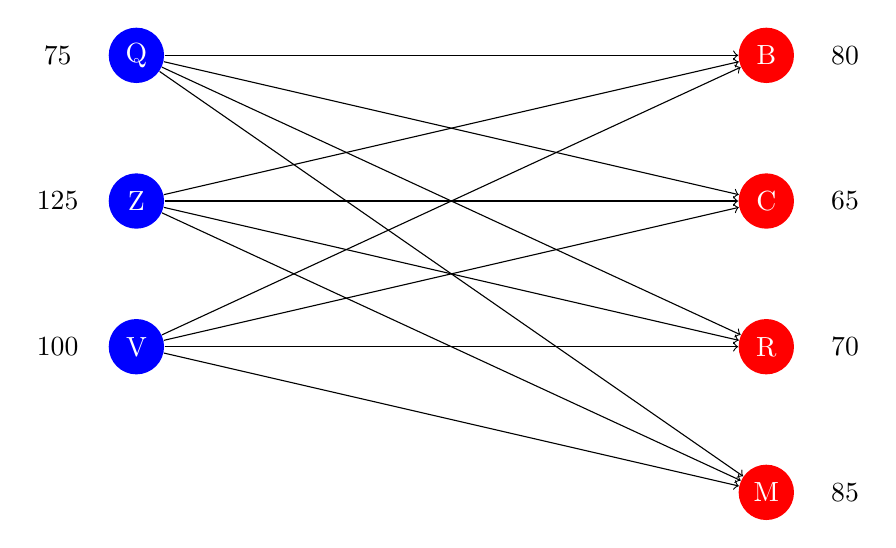
\begin{tikzpicture}

    % Define the left and right vertex positions
    \foreach \i/\num/\nom in {1/75/Q, 2/125/Z, 3/100/V} {
        % Left vertices
        \node[circle, fill=blue, minimum size=20pt, inner sep=0pt, text=white] (L\i) at (-4, -1.85*\i) {\nom};
        % Number to the left of the left vertices
        \node at (-5, -1.85*\i) {\num};
    }
    
    \foreach \i/\num/\nom in {1/B/80, 2/C/65, 3/R/70, 4/M/85} {
        % Right vertices
        \node[circle, fill=red, minimum size=20pt, inner sep=0pt, text=white] (R\i) at (4, -1.85*\i) {\num};
        % Number to the right of the right vertices
        \node at (5, -1.85*\i) {\nom};
    }
    
    % Draw edges between left and right vertices with labels
    \foreach \i in {1, 2, 3} {
        \foreach \j in {1, 2, 3, 4} {
            \draw[->] (L\i) -- (R\j) node[midway, above, sloped] {};
        }
    }
    
    \end{tikzpicture}


  
  \end{frame}

  \begin{frame}[fragile]{Representación gráfica del problema.}
    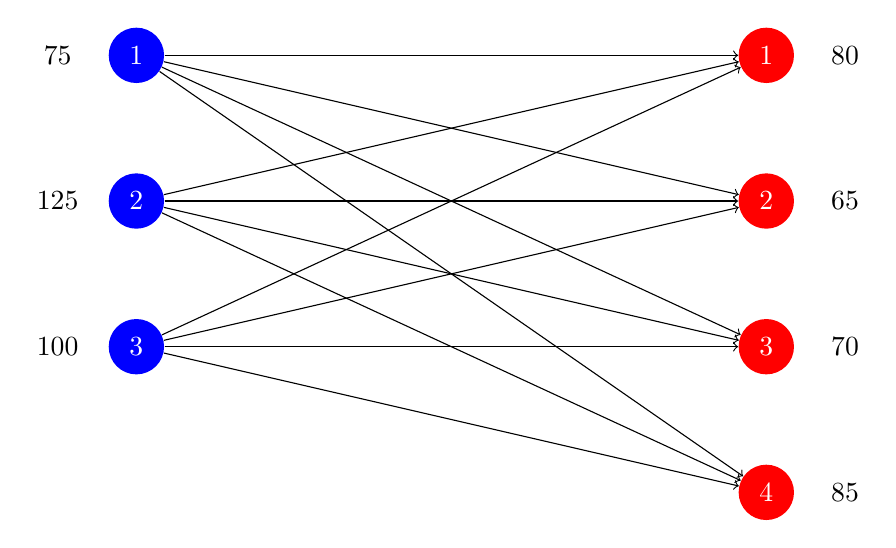
\begin{tikzpicture}

      % Define the left and right vertex positions
      \foreach \i/\num/\nom in {1/1/75, 2/2/125, 3/3/100} {
          % Left vertices
          \node[circle, fill=blue, minimum size=20pt, inner sep=0pt, text=white] (L\i) at (-4, -1.85*\i) {\num};
          % Number to the left of the left vertices
          \node at (-5, -1.85*\i) {\nom};
      }
      
      \foreach \i/\num/\nom in {1/1/80, 2/2/65, 3/3/70, 4/4/85} {
          % Right vertices
          \node[circle, fill=red, minimum size=20pt, inner sep=0pt, text=white] (R\i) at (4, -1.85*\i) {\num};
          % Number to the right of the right vertices
          \node at (5, -1.85*\i) {\nom};
      }
      
      % Draw edges between left and right vertices with labels
      \foreach \i in {1, 2, 3} {
          \foreach \j in {1, 2, 3, 4} {
              \draw[->] (L\i) -- (R\j) node[midway, above, sloped] {};
          }
      }
      
      \end{tikzpicture}
  \end{frame}

  \begin{frame}[fragile]{Formulación matemática del problema: función objetivo.}
    La función de objetivo va a estar dada por 
    \begin{align*}
      Z &= c_{11}x_{11} + c_{12}x_{12} + \dots +  c_{34}x_{34} \\
    \end{align*}
    \pause 
    De forma matricial podemos escribir 
    \caja{Z  = c \cdot x^{t}}

    donde:
    \begin{itemize}
      \item $c = ( 464 , 513 , 654 , 867 , 352 , 416 , 690 , 791 , 995 , 682 , 388 , 685 )$.
      \item $x = (x_{11}, x_{12}, x_{13},x_{14},x_{21}, x_{22}, x_{23},x_{24} ,x_{31}, x_{32}, x_{33}, x_{34})$.
    \end{itemize}
  \end{frame}

  \begin{frame}[fragile]{Formulación matemática del problema: restricciones}
    De la producción obtenemos las siguientes restricciones.
    \begin{align*}
      x_{11} + x_{12} + x_{13} + x_{14} &= 75 \\
      x_{21} + x_{22} + x_{23} + x_{24} &= 125 \\
      x_{31} + x_{32} + x_{33} + x_{34} &= 100 \\
    \end{align*}
    \pause 
    De la demanda obtenemos las siguientes restricciones.
    \begin{align*}
      x_{11} + x_{21} + x_{31} &= 80 \\
      x_{12} + x_{22} + x_{32} &= 65 \\
      x_{13} + x_{23} + x_{33} &= 70 \\
      x_{14} + x_{24} + x_{34} &= 85 \\
    \end{align*}
    \pause 
    Como siempre también tenemos la restricción de no negatividad.
    \[
      x_{ij} \ge 0, \ \ \forall i,j. \ 1 \le i \le 3, \ 1 \le j \le 4
    \]
  \end{frame}
  \begin{frame}[fragile]{Implementación.}
    Pasamos a colab para resolver el problema en Picos.
  \end{frame}

  \begin{frame}[fragile]{Flujo máximo.}
    Una empresa petrolera quiere maximizar la cantidad de petroleo (medido por hora) que sale por conductos del pozo (\emph{source}) y que llega por varios conductos al centro de distribución (\emph{sink}).
    \pause 

    A su vez el petroleo puede pasar posiblemente por tres estaciones: 1,2 y 3.
    Los distintos conductos tienen distintas capacidades máximas.

    \pause 

    Queremos maximizar por hora la cantidad de petroleo que sale del source y llega al sink.
  \end{frame}

  \begin{frame}[fragile]{Capacidad máxima de los conductos.}
    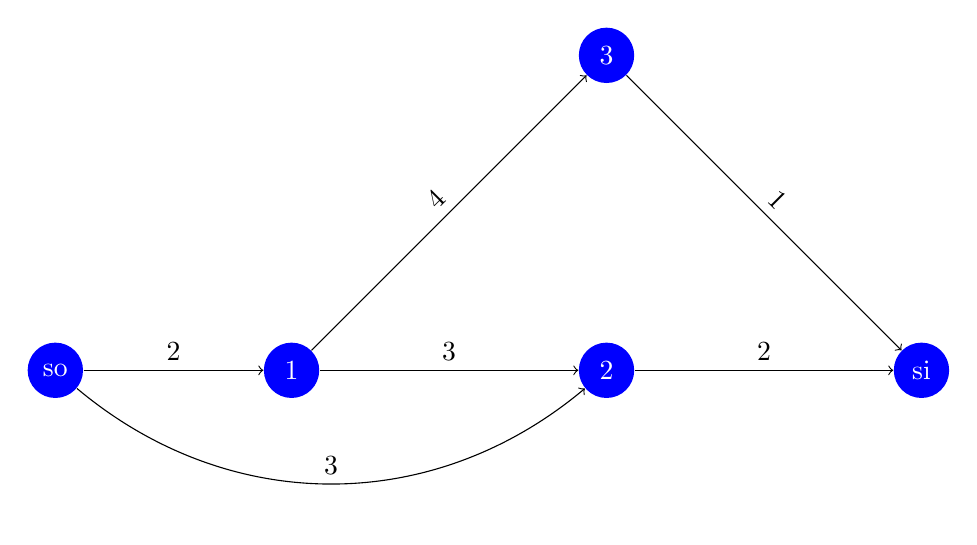
\begin{tikzpicture}
      \node[circle, fill=blue, minimum size=20pt, inner sep=0pt, text=white] (so) at (-5,0) {so};
      \node[circle, fill=blue, minimum size=20pt, inner sep=0pt, text=white] (1) at (-2,0) {1};
      \node[circle, fill=blue, minimum size=20pt, inner sep=0pt, text=white] (2) at (2,0) {2};
      \node[circle, fill=blue, minimum size=20pt, inner sep=0pt, text=white] (3) at (2,4) {3};
      \node[circle, fill=blue, minimum size=20pt, inner sep=0pt, text=white] (si) at (6,0) {si};


      \draw[->] (so) -- (1) node[midway, above, sloped] {$2$};
      \draw[->,bend right=40, label = $3$] (so) to node[midway, above, sloped] {$3$} (2);
      \draw[->] (1) -- (3) node[midway, above, sloped] {$4$};
      \draw[->] (1) -- (2) node[midway, above, sloped] {$3$};
      \draw[->] (2) -- (si) node[midway, above, sloped] {$2$};
      \draw[->] (3) -- (si) node[midway, above, sloped] {$1$};
    \end{tikzpicture}
  \end{frame}

  \begin{frame}[fragile]{Variables de decisión.}
    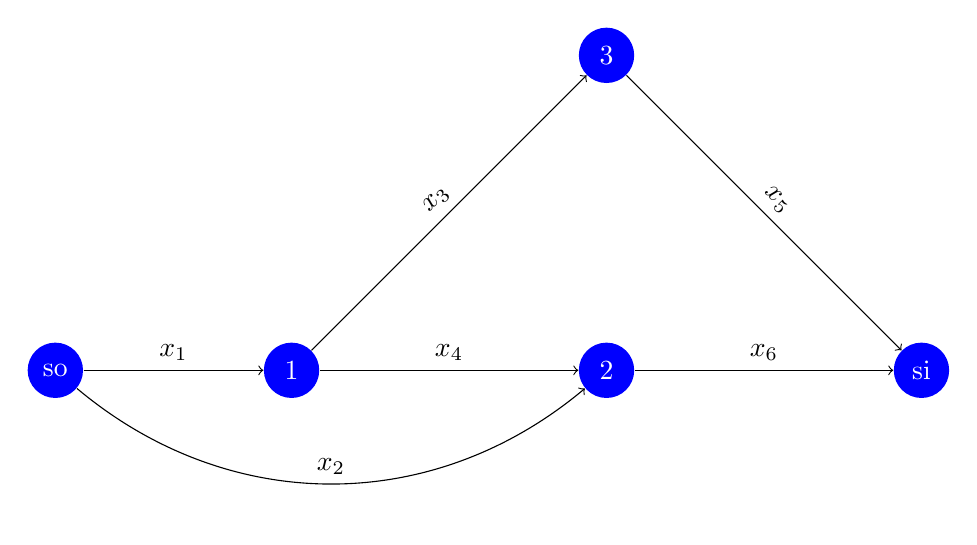
\begin{tikzpicture}
      \node[circle, fill=blue, minimum size=20pt, inner sep=0pt, text=white] (so) at (-5,0) {so};
      \node[circle, fill=blue, minimum size=20pt, inner sep=0pt, text=white] (1) at (-2,0) {1};
      \node[circle, fill=blue, minimum size=20pt, inner sep=0pt, text=white] (2) at (2,0) {2};
      \node[circle, fill=blue, minimum size=20pt, inner sep=0pt, text=white] (3) at (2,4) {3};
      \node[circle, fill=blue, minimum size=20pt, inner sep=0pt, text=white] (si) at (6,0) {si};


      \draw[->] (so) -- (1) node[midway, above, sloped] {$x_{1}$};
      \draw[->,bend right=40, label = $3$] (so) to node[midway, above, sloped] {$x_{2}$} (2);
      \draw[->] (1) -- (3) node[midway, above, sloped] {$x_{3}$};
      \draw[->] (1) -- (2) node[midway, above, sloped] {$x_{4}$};
      \draw[->] (2) -- (si) node[midway, above, sloped] {$x_{6}$};
      \draw[->] (3) -- (si) node[midway, above, sloped] {$x_{5}$};
    \end{tikzpicture}
  \end{frame}

  \begin{frame}[fragile]{Formulación matemática del problema.}
    Nuestra función objetivo a \emph{maximizar} es la siguiente:
    \[
      Z = x_{1} + x_{2}
    \]
    \pause 

    \begin{itemize}
      \item Que corresponde al flujo total de la red (desde el punto de vista matemático).
      \item Que corresponde a la cantidad de petroleo que podemos extraer del pozo y hacer que llegue a nuestro objetivo (desde el punto de vista práctico).
    \end{itemize}
  \end{frame}

  \begin{frame}[fragile]{Restricciones}
    Todo problema de flujo tiene los siguientes invariantes que se deben satisfacer.
    \begin{itemize}
      \item Cada nodo intermedio (en nuestro caso los nodos correspondientes a las estaciones 1,2,3), todo el petroleo que entra debe salir. 
      \item Cada conducto tiene una capacidad máxima.
    \end{itemize}
  \end{frame}

  \begin{frame}[fragile]{Restricciones}
    De esta manera tenemos las siguientes restricciones.

    \begin{align*}
      \text{Nodo 1} & \to & x_{1} &= x_{3} + x_{4} \\
      \text{Nodo 2} & \to & x_{4} + x_{2} &= x_{6} \\
      \text{Nodo 1} & \to & x_{3} &= x_{5} \\
    \end{align*}

    \pause 
    \bigskip 

    Por otro lado las variables están acotadas de la siguiente manera.

    \begin{align*}
      0 \le x_{1} \le 2 & &0 \le x_{2} \le 3 \\
      0 \le x_{3} \le 4 & &0 \le x_{4} \le 3 \\
      0 \le x_{5} \le 1 & &0 \le x_{6} \le 2 \\
    \end{align*}
  \end{frame}

  \begin{frame}[fragile]{Solución.}
    Verificar (programandolo o sino mirando mi solución) que la siguiente es la respuesta al problema de flujo máximo.

    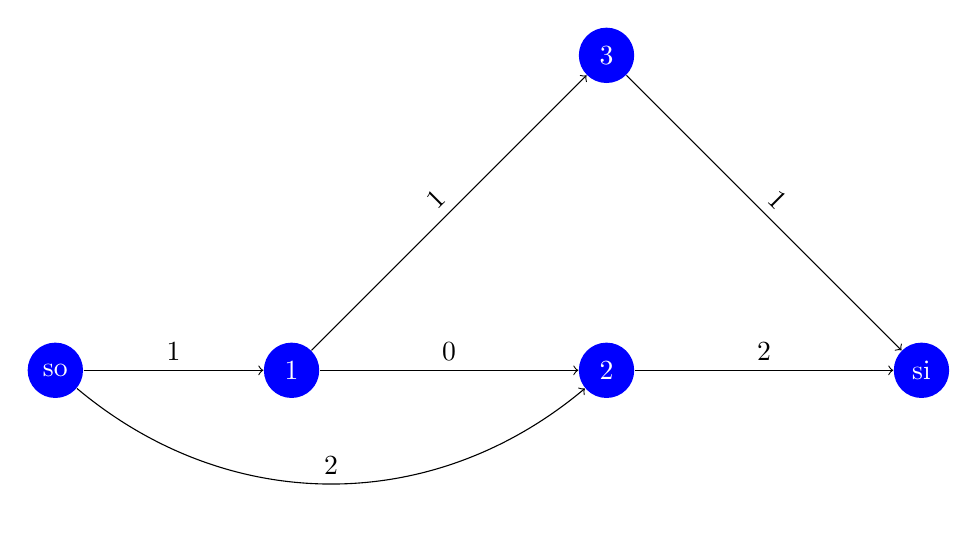
\begin{tikzpicture}
      \node[circle, fill=blue, minimum size=20pt, inner sep=0pt, text=white] (so) at (-5,0) {so};
      \node[circle, fill=blue, minimum size=20pt, inner sep=0pt, text=white] (1) at (-2,0) {1};
      \node[circle, fill=blue, minimum size=20pt, inner sep=0pt, text=white] (2) at (2,0) {2};
      \node[circle, fill=blue, minimum size=20pt, inner sep=0pt, text=white] (3) at (2,4) {3};
      \node[circle, fill=blue, minimum size=20pt, inner sep=0pt, text=white] (si) at (6,0) {si};


      \draw[->] (so) -- (1) node[midway, above, sloped] {$1$};
      \draw[->,bend right=40, label = $3$] (so) to node[midway, above, sloped] {$2$} (2);
      \draw[->] (1) -- (3) node[midway, above, sloped] {$1$};
      \draw[->] (1) -- (2) node[midway, above, sloped] {$0$};
      \draw[->] (2) -- (si) node[midway, above, sloped] {$2$};
      \draw[->] (3) -- (si) node[midway, above, sloped] {$1$};
    \end{tikzpicture}

    Es decir el flujo máximo es $3$.
  \end{frame}

  \begin{frame}[fragile]{Tarea.}
    \tcajita{Problema}
    {¿Que pasaría si en el problema de transporte anteriormente visto aumentamos la demanda de bizcochos de Buenos Aires?
    Es decir consideramos el mismo problema de antes pero la tabla de demanda ahora está dada por:
      \begin{center}
        \begin{tabular}{|c|c|c|c|c|}
          \hline
           & B & C & R & M \\
          \hline
          Demanda & \alert{100} & 65 & 70 & 85 \\
          \hline
        \end{tabular}
      \end{center}
    Consideramos la siguiente tabla de costos de demanda insastifecha.
      \begin{center}
        \begin{tabular}{|c|c|c|c|c|}
          \hline
           & B & C & R & M \\
          \hline
          Demanda insastifecha & 1500 & 1200 & 1350 & 990 \\
          \hline
        \end{tabular}
      \end{center}
    Plantear el problema de transporte asociado y resolverlo.
  }
  \end{frame}

\end{document}
